\section{Version \small\LILLYxBOXxVersion{1.0.7}}
\elable{jmp:oldInstallLinux}
\subsection{Installation in Linux}
\LILLYxNOTExVersion{1.0.0}Da LILLY komplett auf einem Linux-Betriebsystem entwickelt wurde, gestaltet sich die Implementierung relativ einfach.
Zuerst gilt es einen neuen Ordner zu erstellen\marginpar{\tiny  Es wird \emph{nicht} auf die Semantik einzelner Befehle eingegangen! Copy\&Paste ist doof, tippen! ;)}:
\begin{lstlisting}[language=lBash]
mkdir -p "${HOME}/texmf/tex/latex/"
\end{lstlisting}
In diesen Ordner (wenn nicht sogar bereits existent) kann nun der gesamte \T{Lilly}-Ordner verschoben werden (oder mithilfe eines symbolischen Links verknüpft). Als letztes muss man nun noch \TeX{} über das neue Verzeichnis informieren:\marginpar{\tiny  Dies sichert uns die Persistenz des Pakets im Falle einer Neuinstallation/Updates von \LaTeX}
\begin{lstlisting}[language=lBash]
texhash "${HOME}/texmf"
\end{lstlisting}

Nun gilt es sich den anderen mitgelieferten Dateien zu widmen! Von besonderer Relevanz ist hierbei \T{lilly\_compile.sh}, welches hier ausführlicher beschrieben wird(REMOVED: OLD). Grundlegend generiert es ein Makefile, das dann zum Kompilieren des Dokuments gedacht ist!\newline
Mithilfe von folgendem Befehl wurde das Makefile für diese Dokumentation generiert:
\begin{lstlisting}[language=lBash]
./lilly_compile.sh "Lilly-Dokumentation.doc.tex" \
                 -dir="Dokumentation/"
\end{lstlisting}
\LILLYxNOTExVersion{1.0.2}Hierbei wird das Makefile gemäß folgenden Regeln erzeugt:
\begin{itemize}[label=$\diamond$]\narrowitems
    \item Es soll die tex-Datei: \say{Lilly-Dokumentation.doc.tex} kompiliert werden.
    \item Das ganze soll (relativ zu \T{lilly\_compile.sh}) im Verzeichnis \T{Dokumentation} stattfinden - hier wird ebenfalls das Makefile generiert. \marginpar{\vspace*{2em}\tiny  Es wird mit den Regeln \T{default, all} und \T{clean} generiert, selbstredend lässt sich dies erweitern}\begin{bemerkung}[make]
        Logischerweise muss damit auch \T{make} auf dem System vorhanden sein:
\begin{lstlisting}[language=lBash]
sudo apt install "make"
\end{lstlisting}
    \end{bemerkung}
\end{itemize}
Mit diesem Makefile kann man nun das Dokument generieren lassen. Zu beachten sei hierbei, dass \T{make} - im Falle der Regel \T{all} - Regeln parallel ausführen wird! \newline
\marginpar{\tiny  Die Anführungszeichen dienen hier und in anderen Codebeispielen lediglich zur Übersicht!}Diese Dokumentation wurde mit folgendem Befehl erstellt:
\begin{lstlisting}[language=lBash]
make "BOXMODE=LIMERENCE"
\end{lstlisting}
Hierbei lässt sich ebenfalls erkennen wie sich noch mit dem Makefile einzelne Komponenten (wie das verwendete Boxdesign) ändern lassen!

\subsection{Spezifikation: Plots}
\elable{jmp:PLOTSSPEC}
{\centering \framebox{\parbox{\linewidth}{\centering Dieser Abschnitt beschreibt die Richtlinien, auf denen Plots in LILLY integriert werden sollen. Es wurden noch keine (Ti\textit{k}Z) basierte Plot-Umgebungen in LILLY integriert.\par}}\vspace*{0.5\baselineskip}\par}
\paragraph{graph-Environment:}
Es soll ein graph-Environment existieren, was auf Basis von PGF das Erstellen folgender Grafiken immens vereinfachen soll:
\[\begin{tabular}{!{\VRule[1pt]}@{\hspace{0.5em}}C{0.5\textwidth}@{\hspace{0.5em}}|@{\hspace{0.5em}}C{0.25\textwidth}@{\hspace{0.5em}}|@{\hspace{0.5em}}C{0.3\textwidth}@{\hspace{0.5em}}!{\VRule[1pt]}}
    \specialrule{1pt}{0pt}{0pt}
    \bfseries Aktuell &\bfseries Ergebnis &\bfseries Wunsch\\
    \specialrule{1pt}{0pt}{0pt}
    {\footnotesize\begin{lstlisting}[language=lLatex,frame=none,breaklines=true]
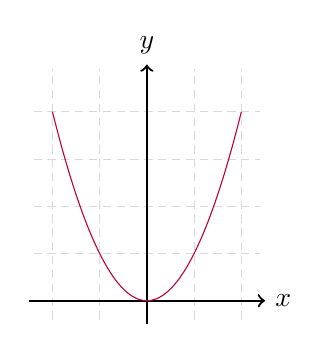
\begin{tikzpicture}[scale=0.6]
    \draw[help lines, color=gray!30,
          densely dashed] (-2.4,-0.4) grid (2.4,4.9);
    \draw[->,thick] (-2.5,0) -- (2.5,0)
          node[right]{$x$};
    \draw[->,thick] (0,-0.5) -- (0,5)
          node[above]{$y$};
    \draw[scale=1,domain=-2:2,
          smooth,variable=\x,purple]
          plot ({\x},{\x*\x});
\end{tikzpicture}
    \end{lstlisting}} &  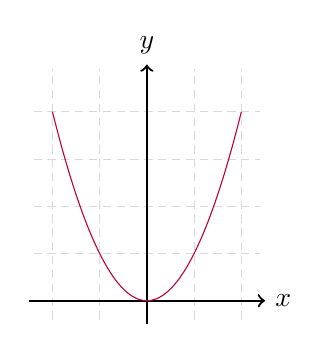
\begin{tikzpicture}[scale=0.6]
        \draw[help lines, color=gray!30,
              densely dashed] (-2.4,-0.4)
              grid (2.4,4.9);
        \draw[->,thick] (-2.5,0) -- (2.5,0)
              node[right]{$x$};
        \draw[->,thick] (0,-0.5) -- (0,5)
              node[above]{$y$};
        \draw[scale=1,domain=-2:2,
              smooth,variable=\x,purple]
              plot ({\x},{\x*\x});
    \end{tikzpicture} &    {\footnotesize\begin{lstlisting}[language=lLatex,frame=none,breaklines=true]
\begin{graph}[scale=0.6,domain=-2:2]
    \plotline[purple]{\x}{\x*\x};
\end{graph}
            \end{lstlisting}}\\
    \specialrule{1pt}{0pt}{0pt}
    \end{tabular}\]
Der Befehl \CMDshow{plotline} soll hierbei nur in der Umgebung verfügbar sein (TODO: gleiches geplant mit PLA etc.).
\paragraph{Positionierung:}
Für die Platzierung von Plots wurden 3 valide Positionen vorgesehen: Zentriert, Links (Text auf rechter Seite), Rechts (Text auf linker Seite). Diese Positionierungen können mithilfe von Floats realisiert werden, sollen aber auf jedenfall auch noch einen absoluten Modus zur Verfügung stellen (primär von zentriert analog zu \verb|\[\]|). Zudem soll das \T{plot}-Environment selbstverständlich auch ohne Positionierung manuell eingebunden werden können!
